\section{Results}
\label{sec:results}

The goal of this section is to quantify the performance of our \ac{LTR} framework when deployed in the environment described in~\autoref{sec:env}.
We achieve this by evaluating the localization accuracy of the \ac{ICP} algorithm through various metrics.
We also show our camera and \ac{GNSS} measurements to demonstrate navigation approaches using these sensors as primary mean of localization would suffer significant performance loss in a subarctic forest.
Afterwards, we evaluate the path-following performance of our controller and quantify our \ac{UGV}'s energy consumption for each run.
Lastly, we identify failure cases for our system and they were handled in the field.

\subsection{Localization}
\label{sec:res_loc}

\lightlipsum[1]

\subsubsection{Vision-based}
\label{sec:res_vis}

The Dalsa C1920 camera allowed us to analyze the feasibility to use this type of sensor in a subarctic forest. As it was observed by ~\citep{Williams2009} and ~\citep{Paton2017}, the use of cameras for robotic purpose in winter conditions is extremely difficult because of the lack of features on snow terrain. As depicted in~\autoref{fig:cameras_b}, the only features available are the ones from the trees and the surroundings. The path totally recovered by snow is flat and without texture.~\citep{Paton2017} also observed that lighting changes can alter the quality of the image and sunlight reflection on snow can saturate the camera sensor. Their observations related to lighting changes was based on the variation of the sun position during the day, but, in our case, the illumination changes inside the same path. In~\autoref{fig:cameras_a}, there is an example from the TeachA where the quality of the image is sufficient while the robot is in the wood, but can drastically changes if there is an opening in the canopy. In those situations, the camera's sensor is overexposed.

Data were also taken during a snowfall to see the effect on image's quality. As we can observed in~\autoref{fig:cameras_b}, snowflakes are circled in red and are practically invisible in the camera image. Another problem with the use of cameras for vision-based localization comes from the lack of luminosity at night as depicted in~\autoref{fig:cameras_c}. The robot needs to be equipped with its own source of light to travel in the dark compared to lidar which is independent to the lighting conditions.

\begin{figure}[htpb]
	\begin{center}
		\begin{subfigure}[b]{0.32\textwidth}
			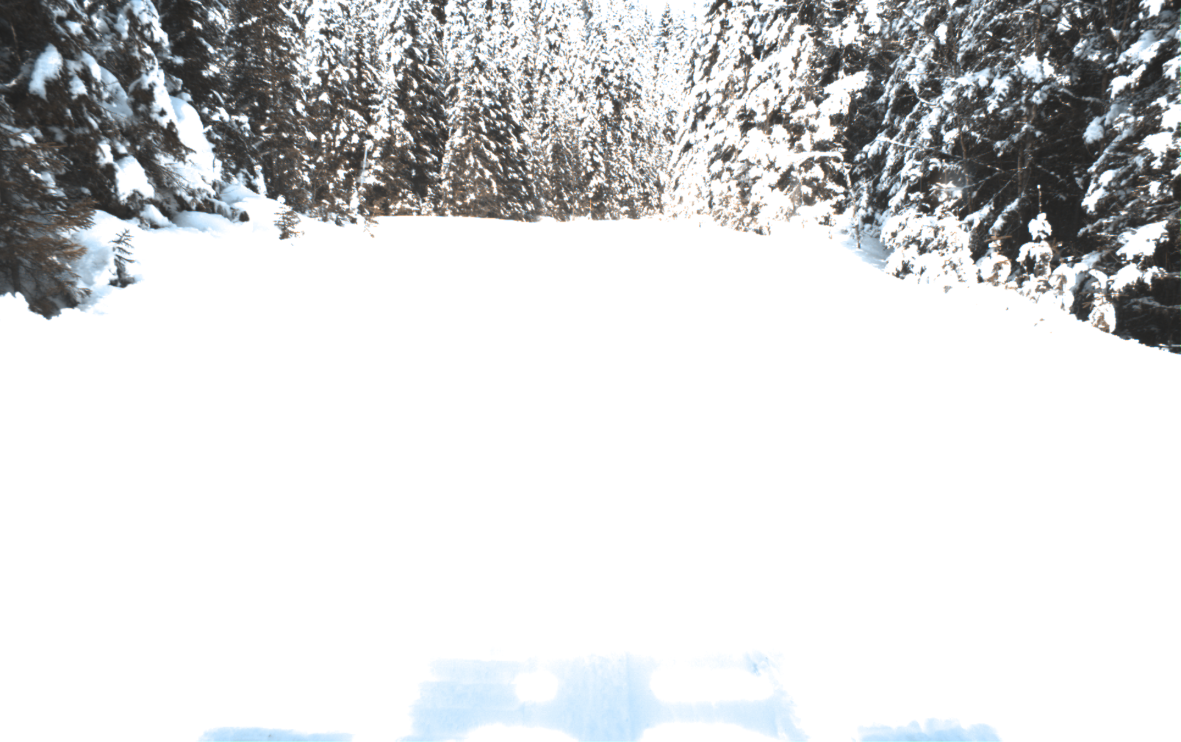
\includegraphics[width=\linewidth]{figs/camera/figure_camera_teachA_top.pdf}
		\end{subfigure}%
		~
		\begin{subfigure}[b]{0.32\textwidth}
			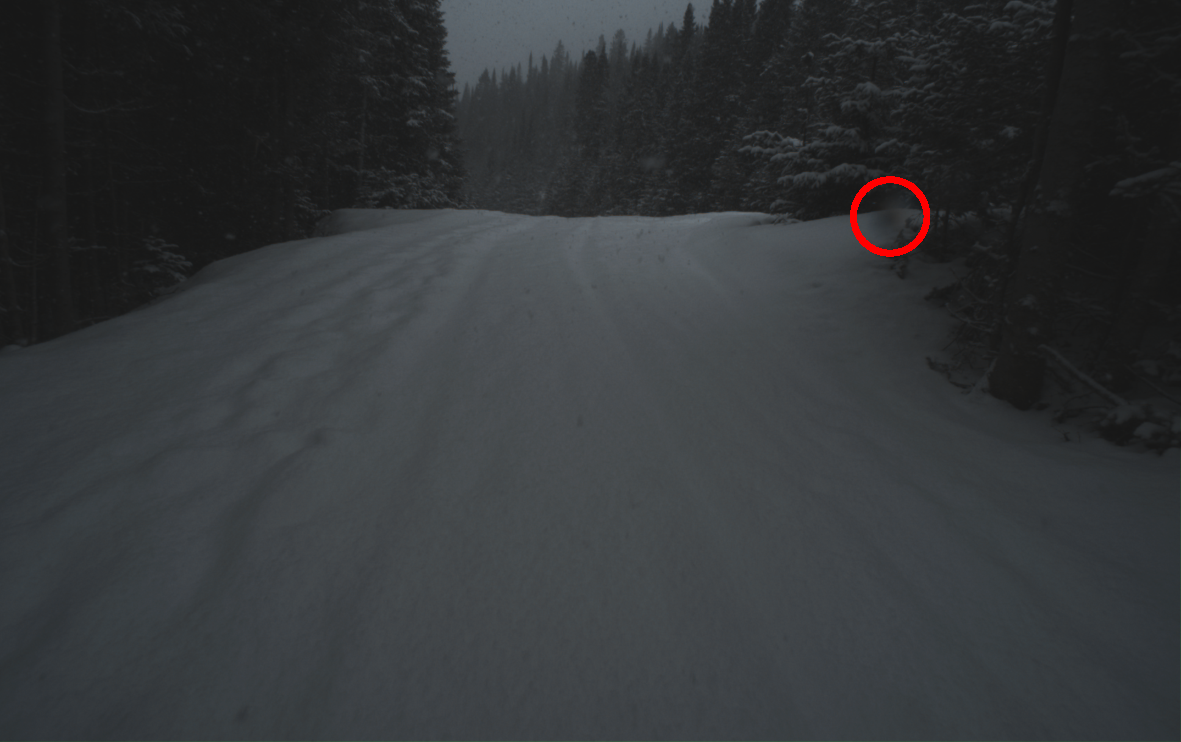
\includegraphics[width=\linewidth]{figs/camera/figure_camera_run9_top.pdf}
		\end{subfigure}
		~
		\begin{subfigure}[b]{0.32\textwidth}
			\includegraphics[width=\linewidth]{figs/camera/figure_camera_dark_top.pdf}
		\end{subfigure}%
		\\ \vspace{2mm}
		\begin{subfigure}[b]{0.32\textwidth}
			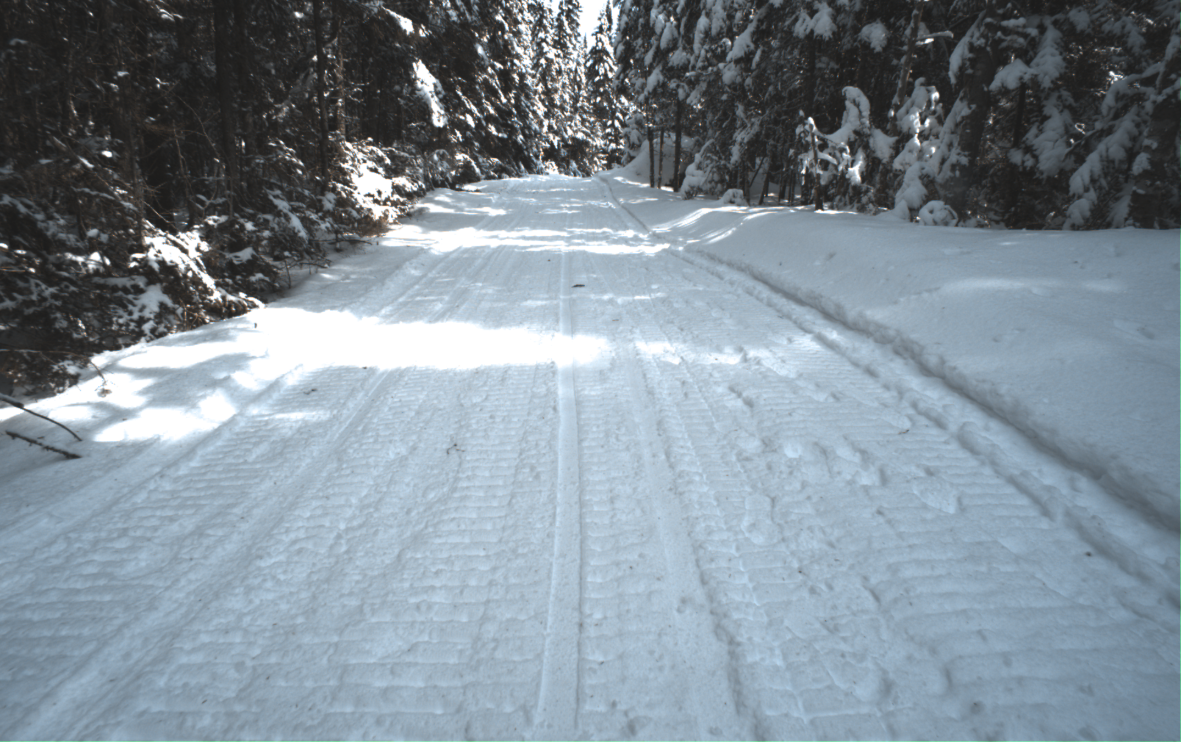
\includegraphics[width=\linewidth]{figs/camera/figure_camera_teachA_bottom.pdf}
			\caption{TeachA}
			\label{fig:cameras_a}
		\end{subfigure}%
		~
		\begin{subfigure}[b]{0.32\textwidth}
			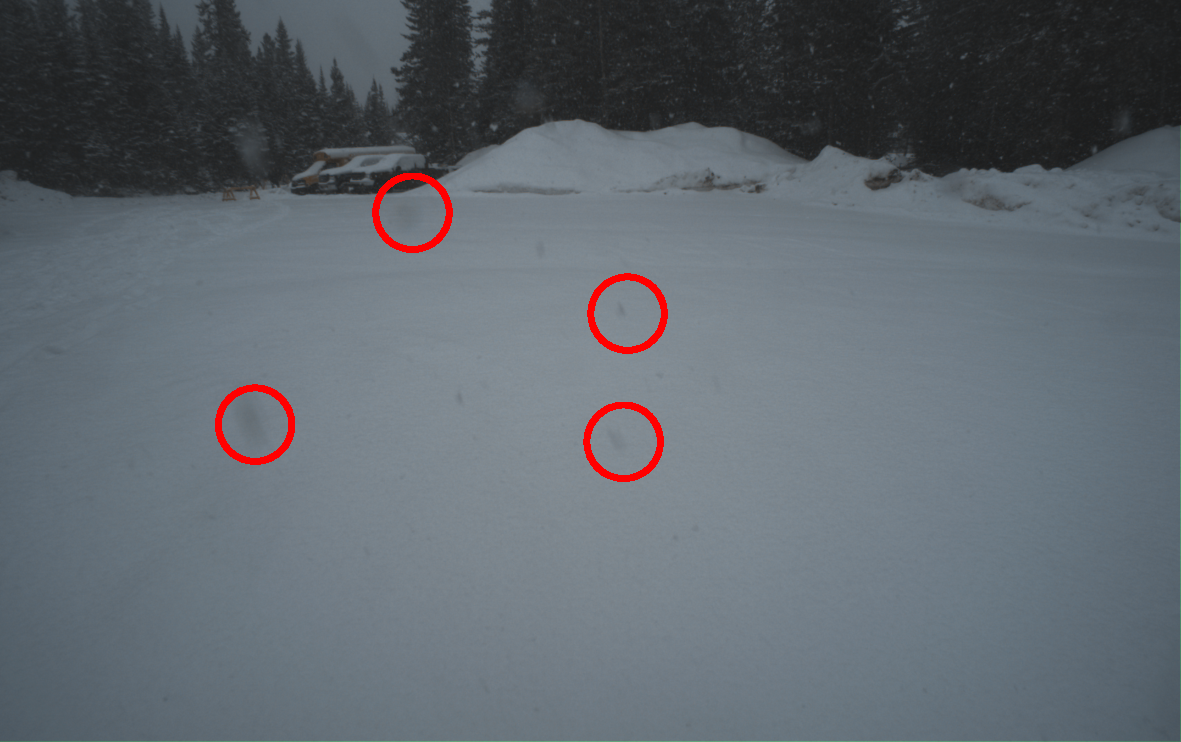
\includegraphics[width=\linewidth]{figs/camera/figure_camera_run9_bottom.pdf}
			\caption{R8}
			\label{fig:cameras_b}
		\end{subfigure}
		~
		\begin{subfigure}[b]{0.32\textwidth}
			
\includegraphics[width=\linewidth]{figs/camera/figure_camera_dark_bottom.pdf}
			\caption{Night}
			\label{fig:cameras_c}
		\end{subfigure}%
	\caption{Pictures taken for three different runs. (a) is an example of the sun's effect on the quality of the images. (b) were taken during a snowfall (most prominent snowflakes are circled in red). Images depicted in (c) were taken at night, hence the lack of luminosity.} 
	\label{fig:cameras_expo}
	\end{center}
\end{figure}

\subsubsection{GNSS}
\label{sec:res_gnss}

\lightlipsum[1]

\begin{figure} [htpb]
	\centering
	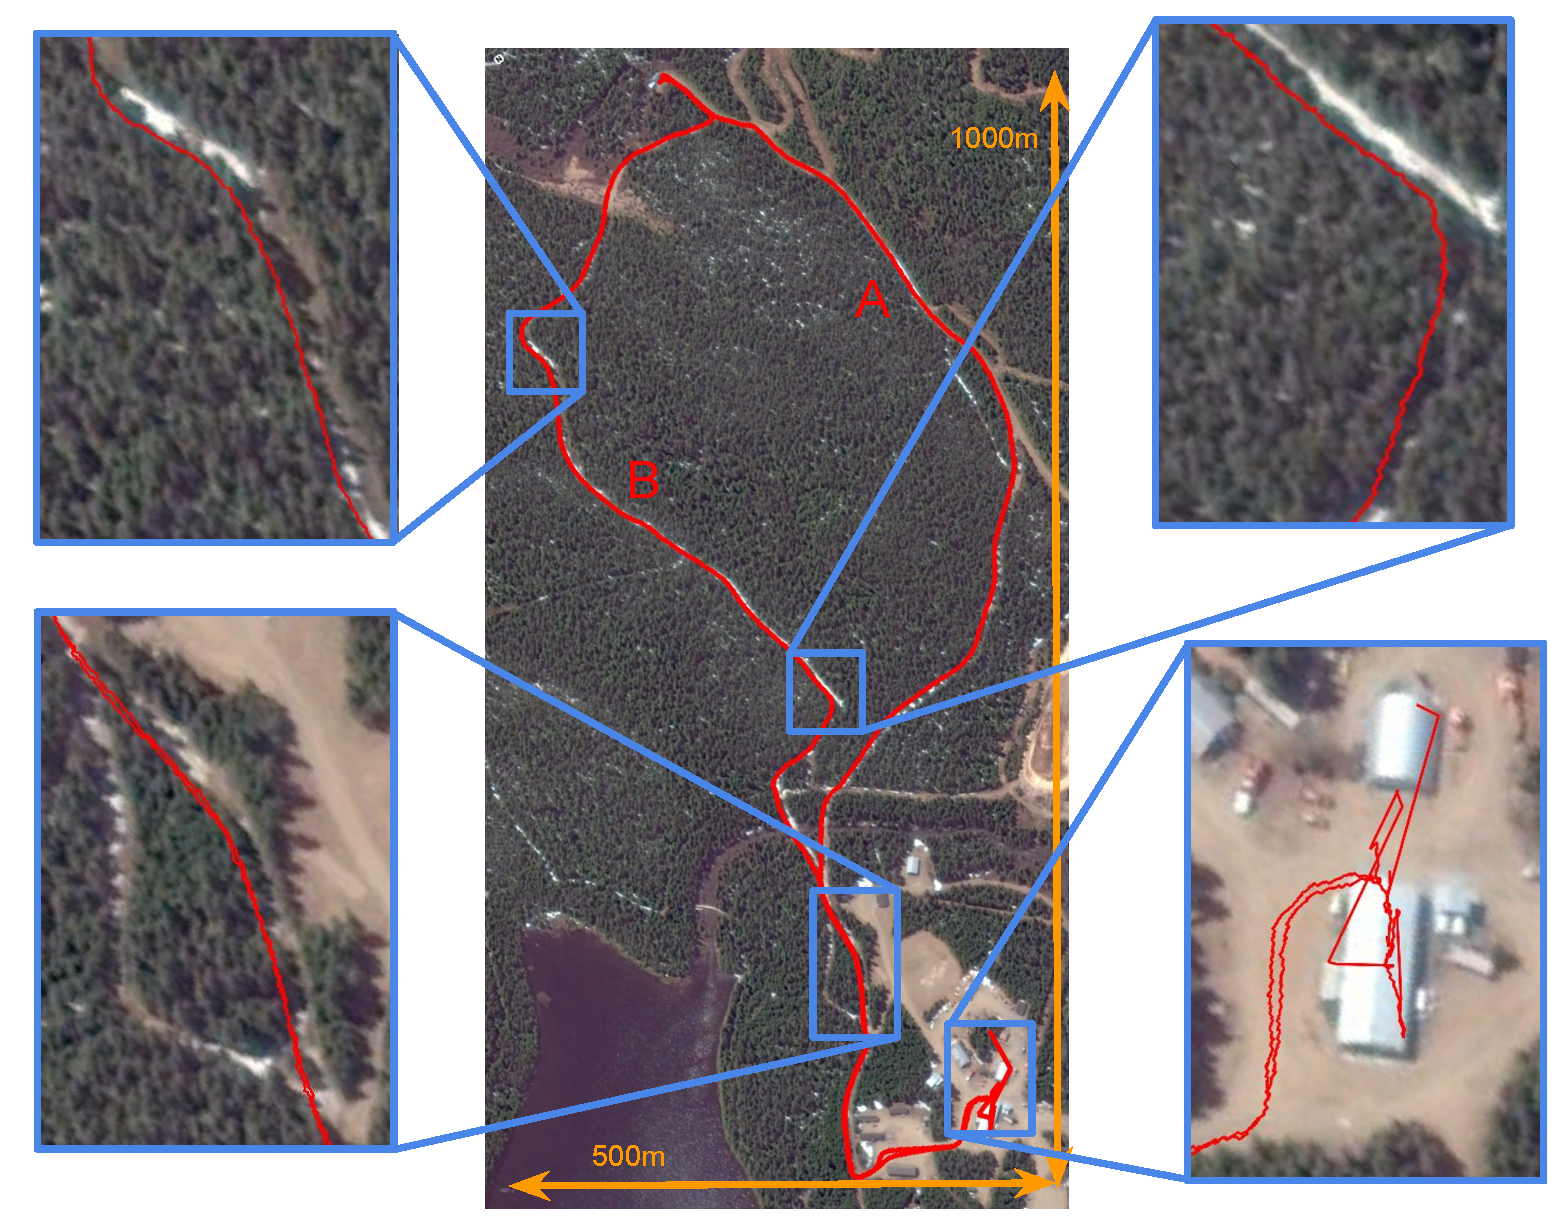
\includegraphics[height=4.0in]{./figs/GPS/FR_gps_data_fails2.pdf}
	\caption{Examples of GPS positioning error along the path A and B.}
	\label{fig:gnss_error_path}
\end{figure}

\begin{figure} [htpb]
	\centering
	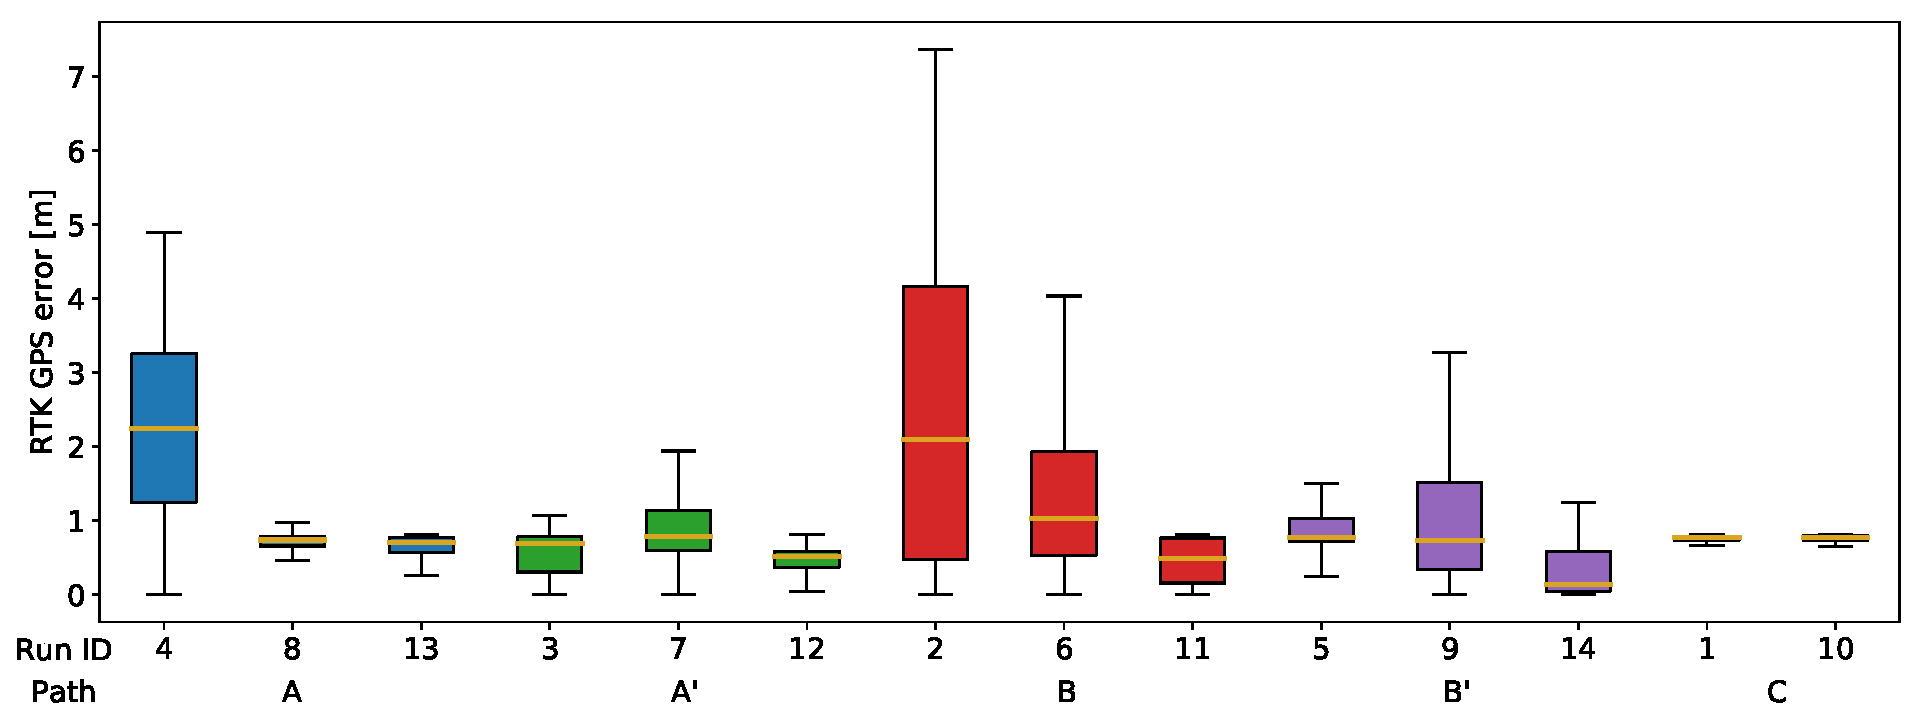
\includegraphics[height=2.0in]{./figs/GPS/RTK_error.pdf}
	\caption{GNSS error for each runs.}
	\label{fig:gnss_run_error}
\end{figure}

\begin{figure} [htpb]
	\centering
	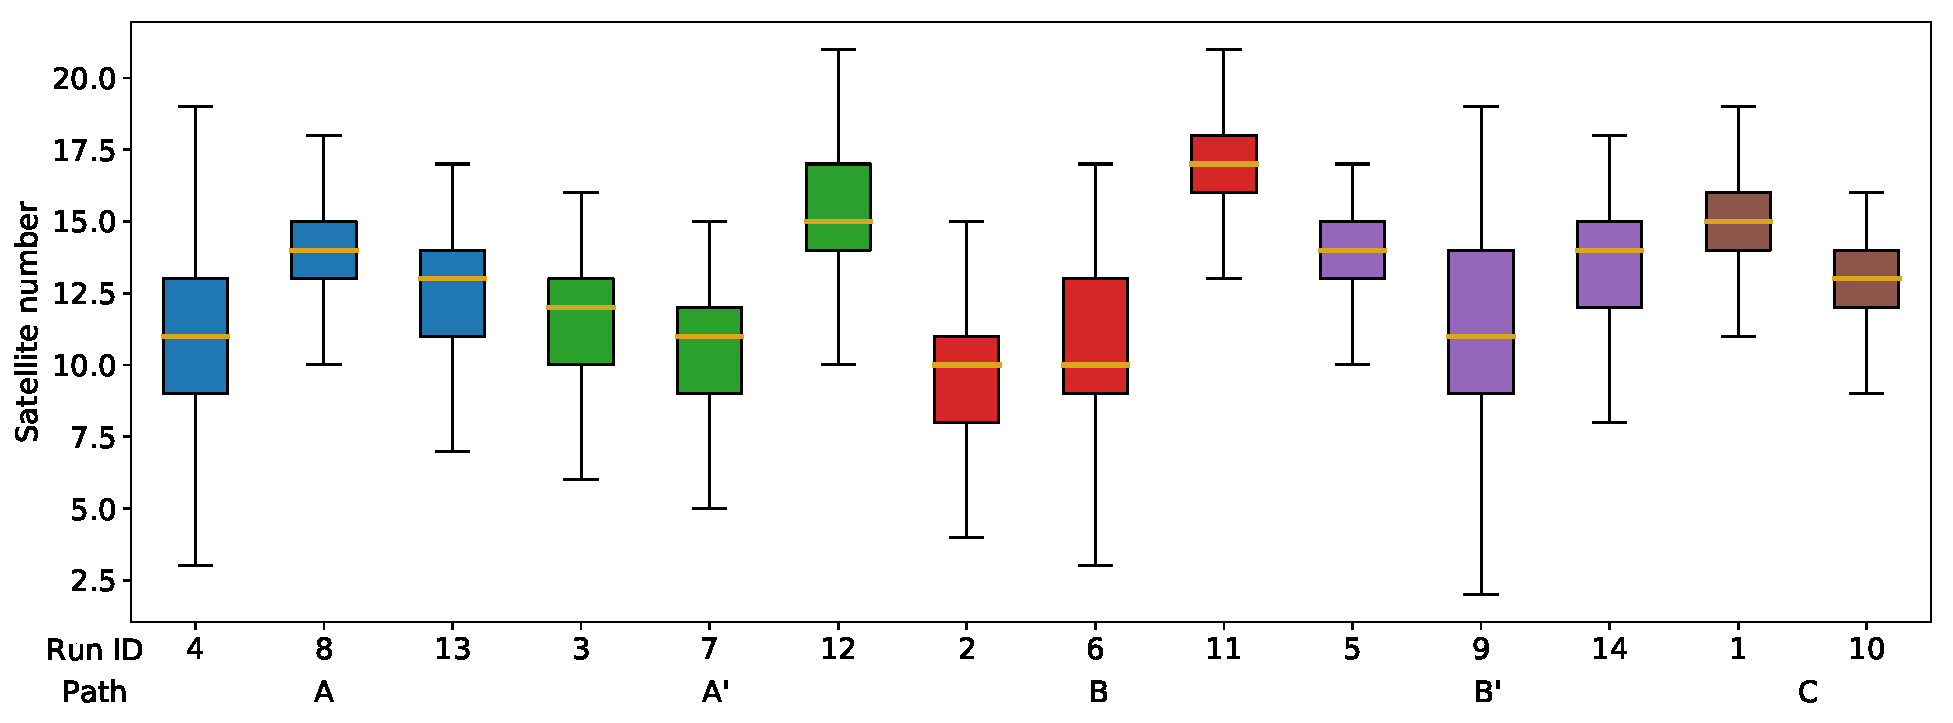
\includegraphics[height=2.0in]{./figs/GPS/Satellite_number.pdf}
	\caption{GNSS satellite number for each run.}
	\label{fig:gnss_satellite_number}
\end{figure}

\subsubsection{ICP}
\label{sec:ICP}

\lightlipsum[1]

\begin{figure} [htpb]
	\centering
	\includegraphics[height=2.0in]{example-image}
	\caption{Figure explaining ICP error for every run (correlated with meteo).}
	\label{fig:icp_error}
\end{figure}



\subsection{Motion and control}
\label{sec:res_motion}

In order to characterize the performance of our path-following controller, we computed the cross track error for each measured position in each repeat run.
Our definition of the cross-track error is the distance between the robot frame $\robotf$'s origin and it's orthogonal projection on the path, as defined in~\citep{Mondoloni2005}.
The results for the cross-track error are displayed in~\autoref{fig:pf_error}.
It can be seen that for all trajectories, the cross-track error mostly remains below \SI{0.1}{m} for most of the runs.
Path curvature can be correlated with an increased cross-track error, with a maximum observed error of \SI{0.8}{m}.
In terms of different runs, it can be observed that cross-track error is stable, despite varying meteorological conditions. 

\begin{figure}[htpb]
	\begin{center}
		\begin{subfigure}[b]{\textwidth}
			\centering
			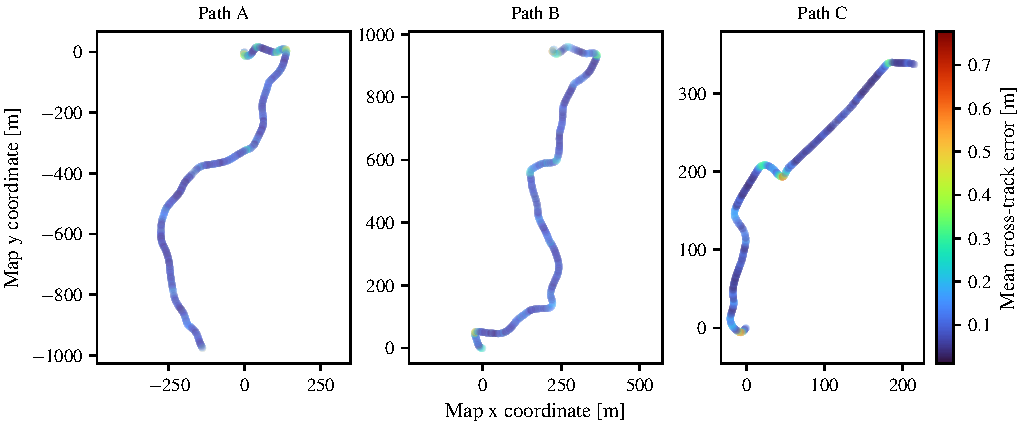
\includegraphics[height=2.5in]{figs/ref_traj_errors.pdf}
			\caption{Mean cross-track error with respect to the reference trajectories.}
			\label{fig:pf_error_traj}
		\end{subfigure}
		\\
		\begin{subfigure}[b]{\textwidth}
			\centering
			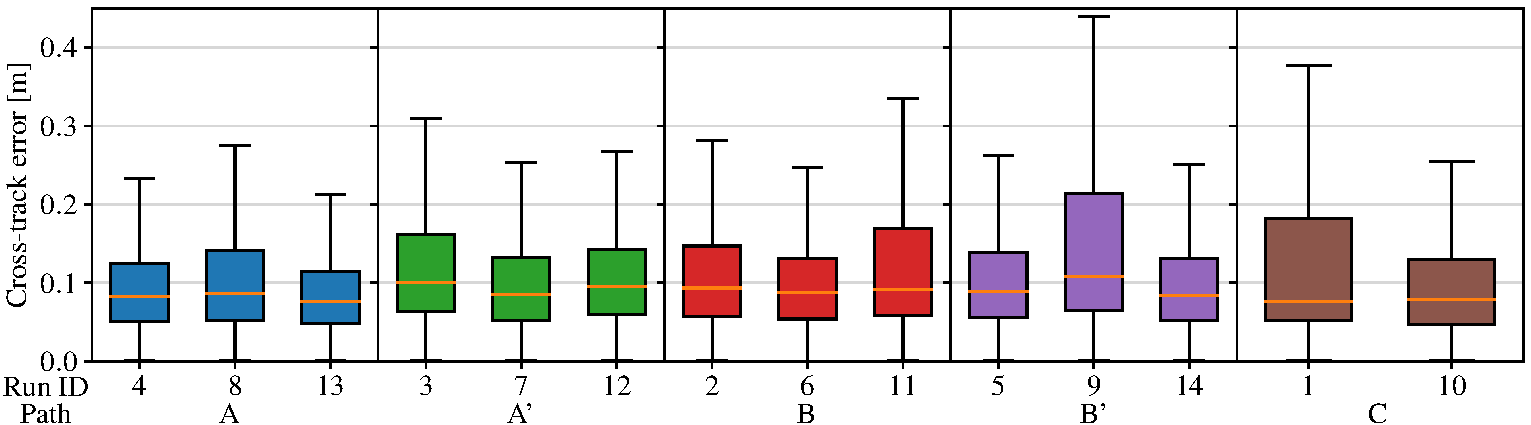
\includegraphics[height=1.6in]{figs/pf_error_runs.pdf}
			\caption{Cross-track error for all runs.}
			\label{fig:pf_error_runs}
		\end{subfigure}
		\caption{Cross-track error during the deployment.
		The cross-track error was computed for every localization position recorded during each repeat run.
		For each map, the coordinates are defined in the reference map frame $\mapf$, which are the same as shown in~\autoref{fig:ref_ltr}.} 
		\label{fig:pf_error}
	\end{center}
\end{figure}


\begin{figure} [htpb]
	\centering
	\includegraphics[height=2.0in]{example-image}
	\caption{Power consumption / motion efficiency figure.}
	\label{fig:moiton_power}
\end{figure}

\subsection{Failure cases}
\label{sec:fail}
%% Discuss Laverdiere failure and garage failure

\subsubsection{Run 2 initialization}
\label{sec:laverdiere_fail}

\lightlipsum[1]

\subsubsection{Run 10 failed initialization}
\label{sec:laverdiere_fail}

\lightlipsum[1]

\begin{figure}[tpbh!]
	\begin{center}
		\begin{subfigure}[b]{0.3\textwidth}
			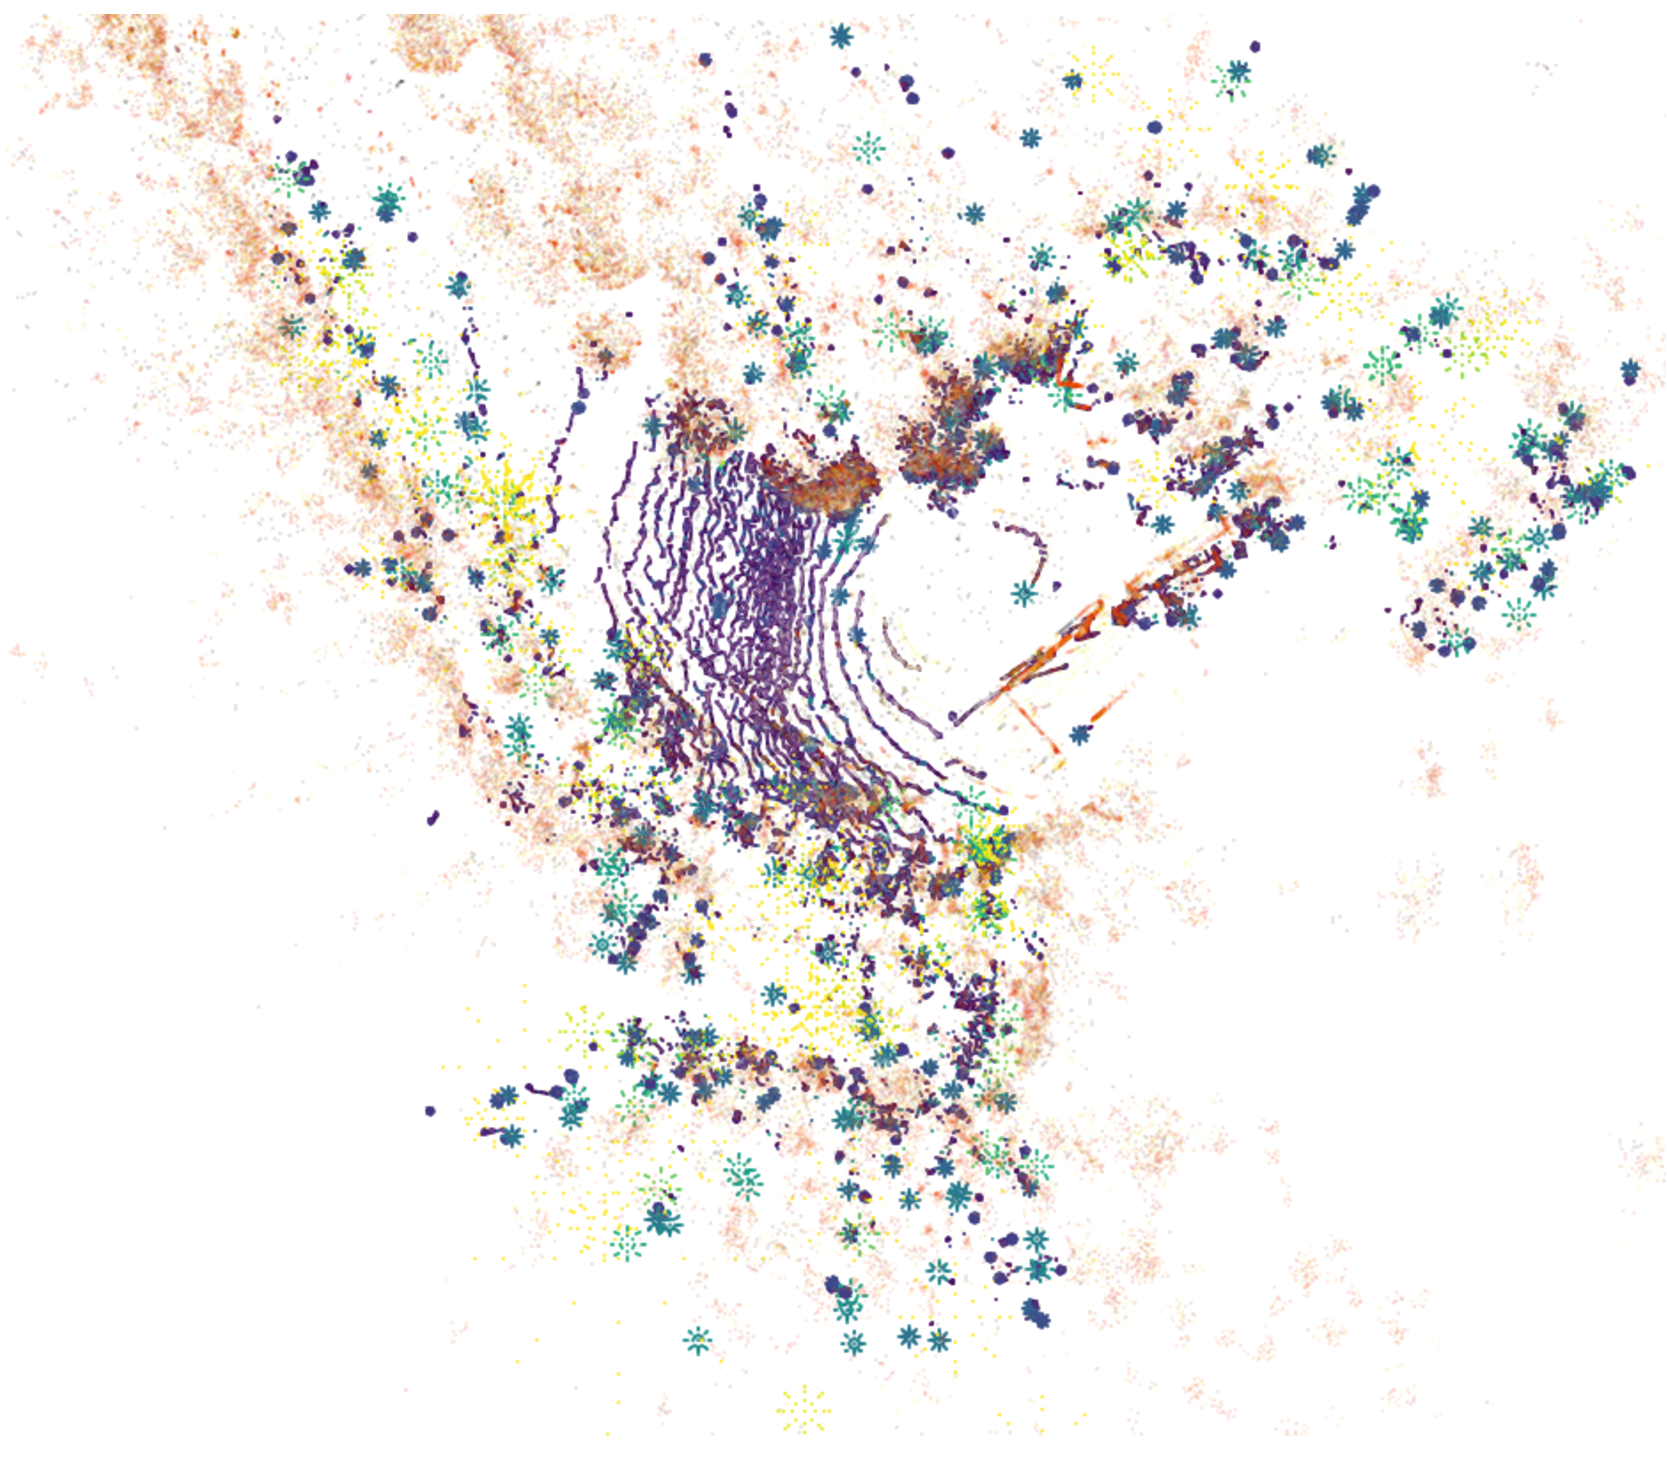
\includegraphics[width=\linewidth]{figs/run10_init_fail/run_6.pdf}
			%\caption{A view from above the \textit{Montmorency} forest, which covers \SI{400}{km^2}.}
			\label{fig:r6_pcl}
			\caption{R6 (Mean error = \SI{0.0607}{m})}
			\vspace{0.2in}
		\end{subfigure}%
		~
		\begin{subfigure}[b]{0.3\textwidth}
			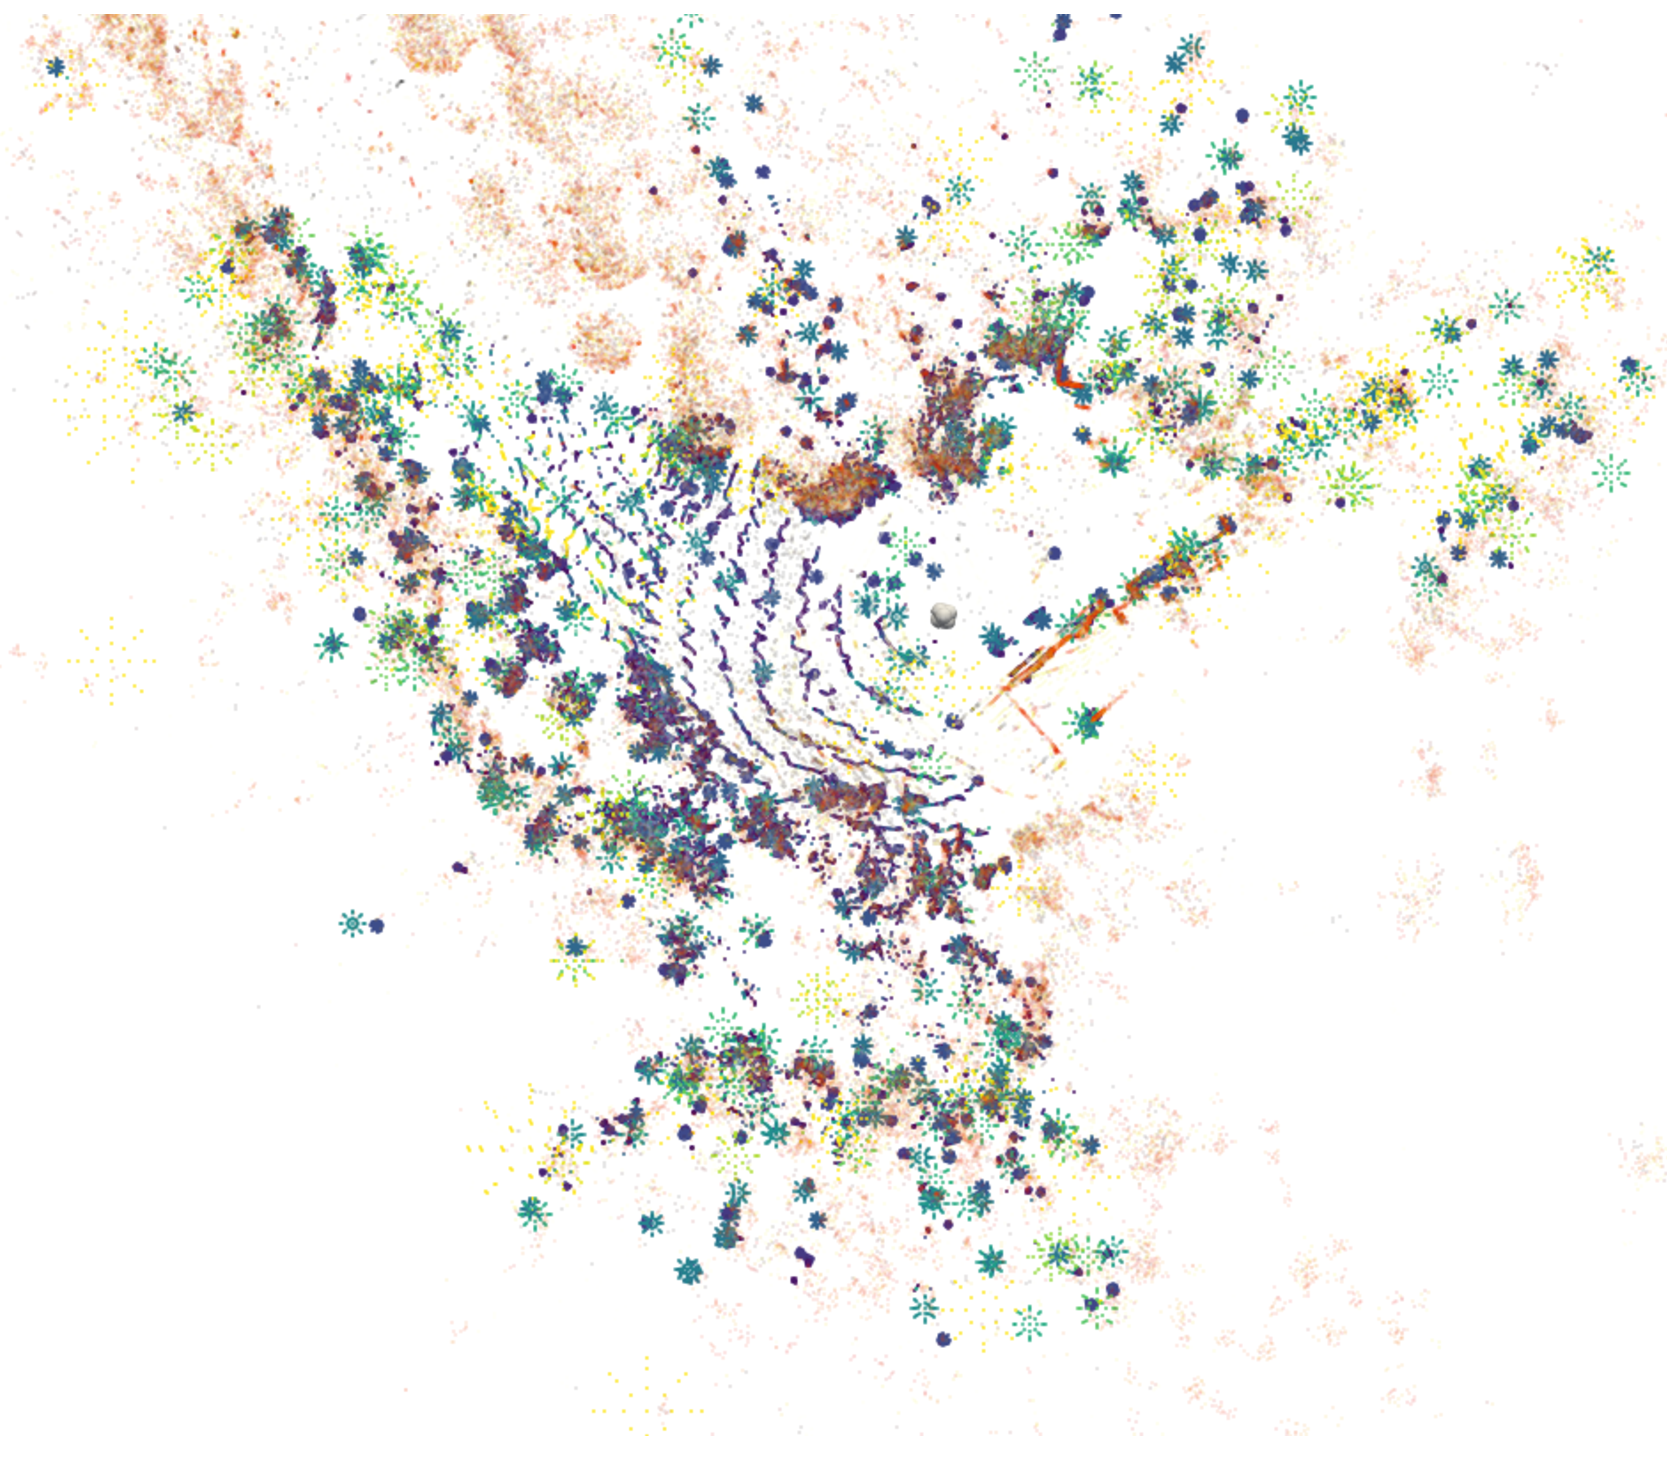
\includegraphics[width=\linewidth]{figs/run10_init_fail/run_10.pdf}
			%\caption{An example of a snowy path, in which our system performed \ac{LTR}.}
			\label{fig:r10_pcl}
			\caption{R10 (Mean error = \SI{0.1072}{m})}
			\vspace{0.2in}
		\end{subfigure}%
		~
		\begin{subfigure}[b]{0.3\textwidth}
			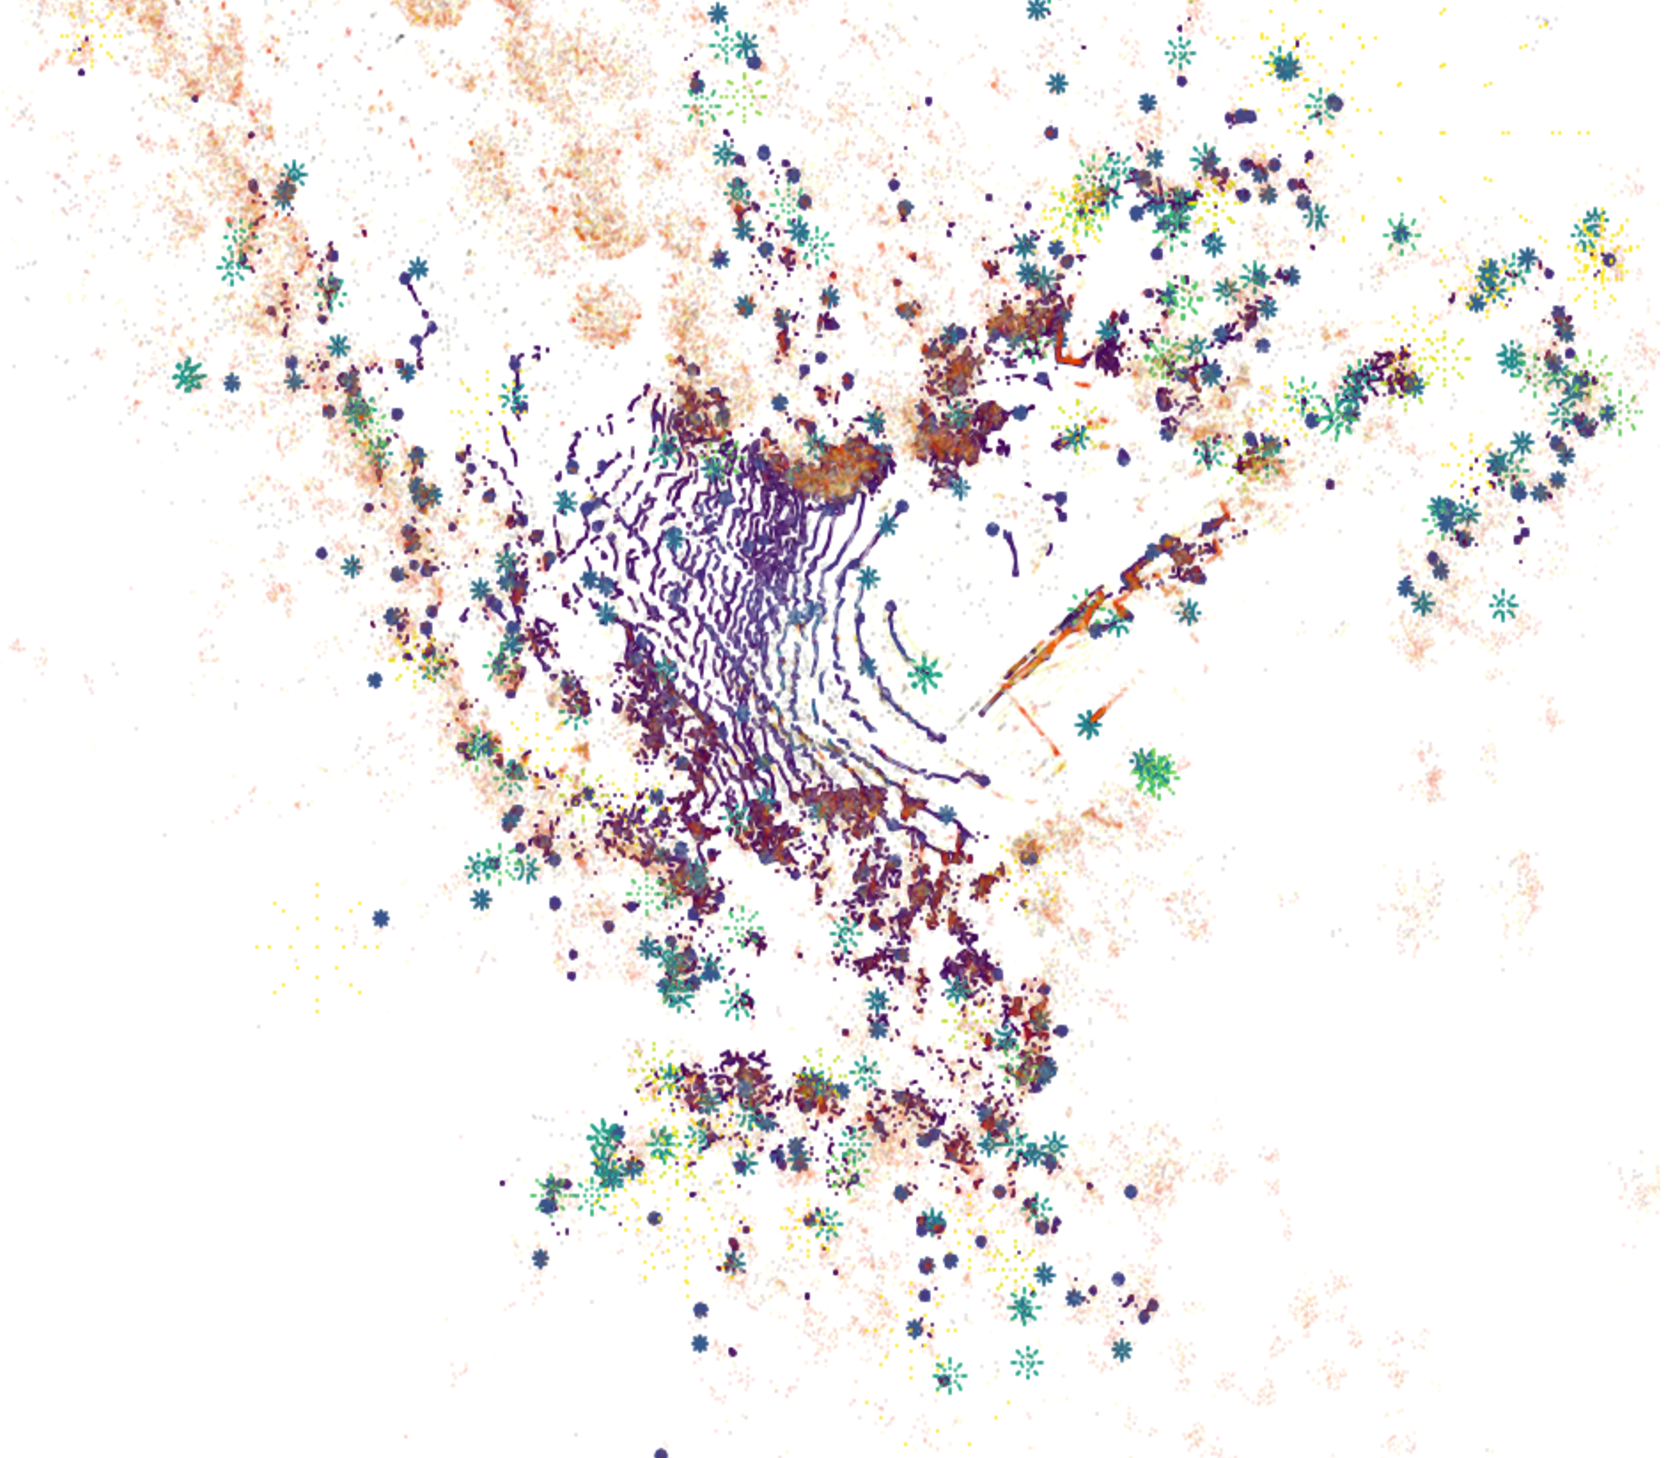
\includegraphics[width=\linewidth]{figs/run10_init_fail/run_15.pdf}
			%\caption{An example of a snowy path, in which our system performed \ac{LTR}.}
			\label{fig:r15_pcl}
			\caption{R15 (Mean error = \SI{0.0698}{m})}
			\vspace{0.2in}
		\end{subfigure}%
		~
		\begin{subfigure}[b]{0.07\textwidth}
			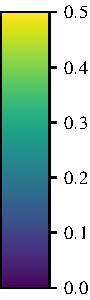
\includegraphics[width=\linewidth]{figs/run10_init_fail/colorbar.pdf}
			%\caption{An example of a snowy path, in which our system performed \ac{LTR}.}
			\label{fig:cbar_run10}
			\vspace{0.2in}
		\end{subfigure}%
		\\
		\begin{subfigure}[b]{0.45\textwidth}
			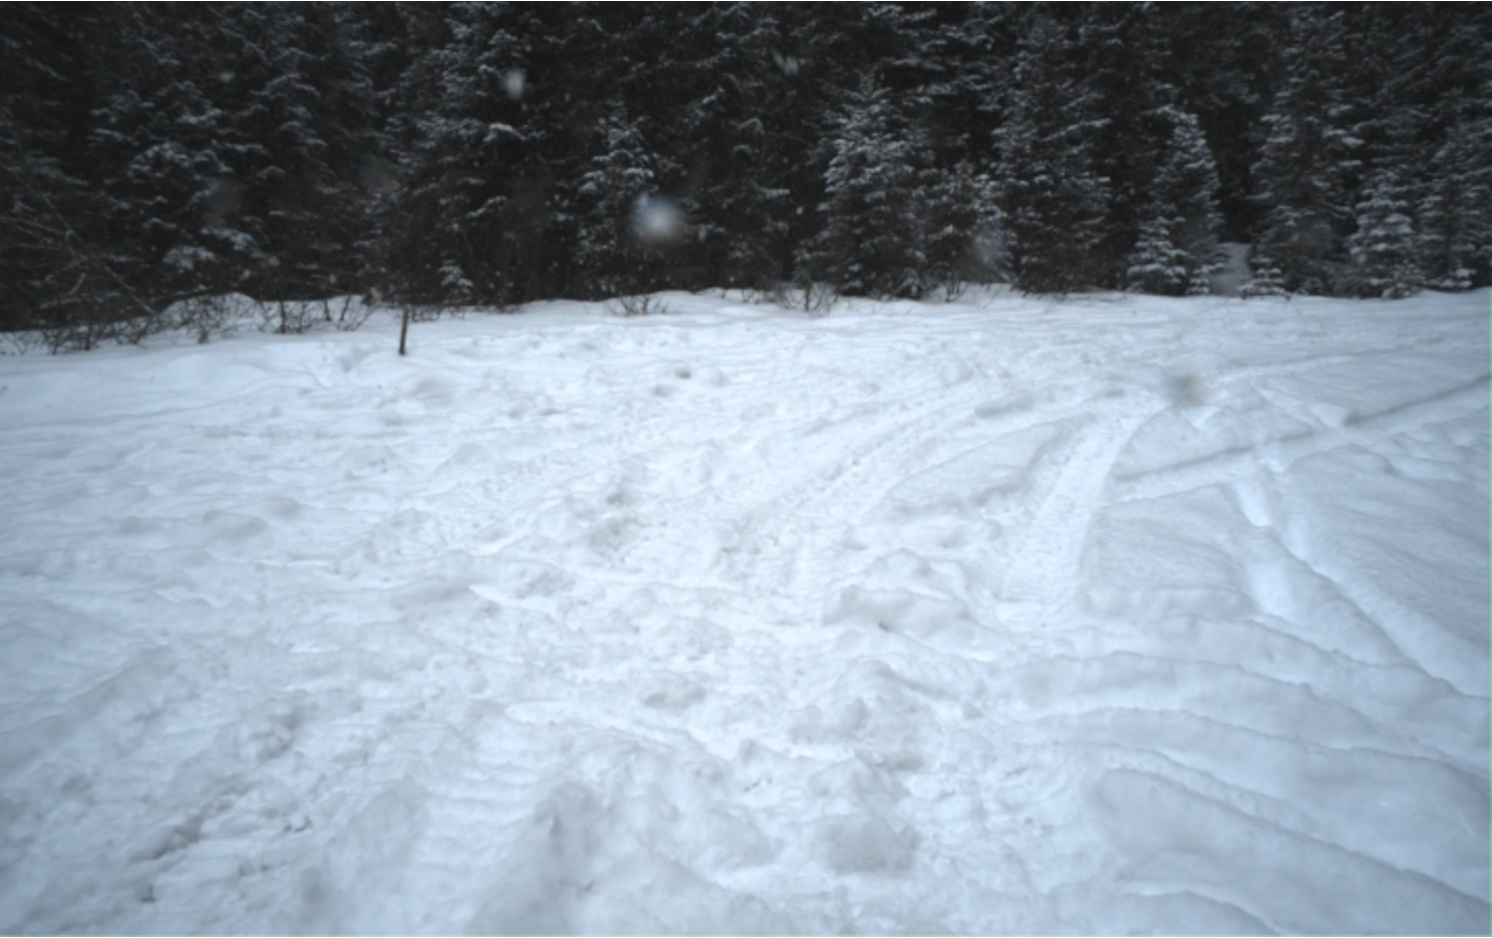
\includegraphics[width=\linewidth]{figs/run10_init_fail/run10_init.pdf}
			\caption{Camera view of R10 initialization.}
			\label{fig:r10_cam}
		\end{subfigure}%
		~
		\begin{subfigure}[b]{0.45\textwidth}
			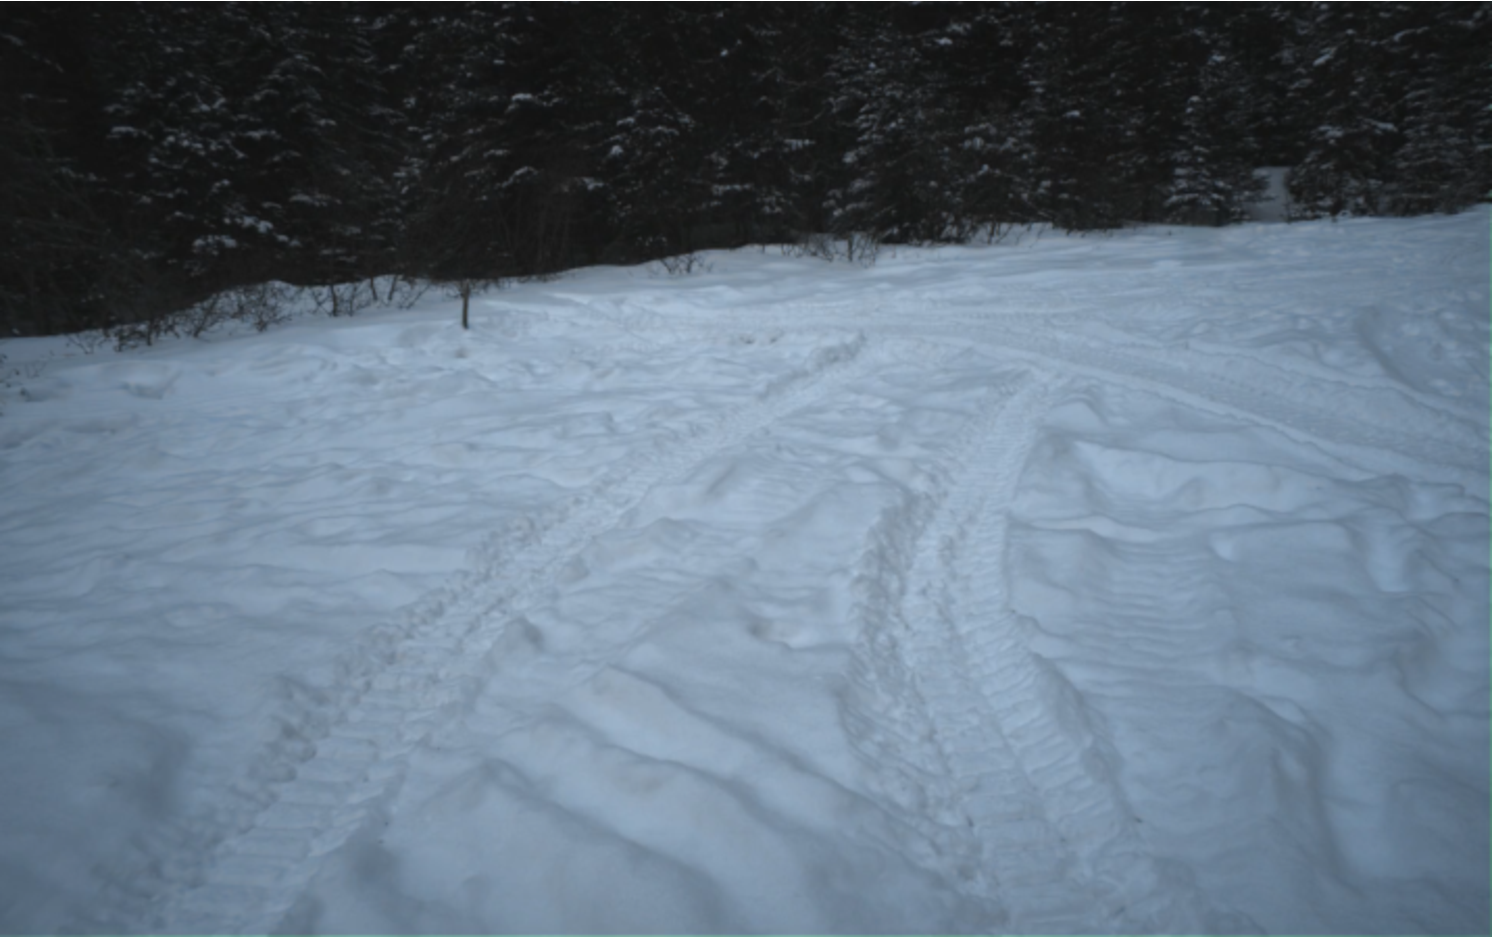
\includegraphics[width=\linewidth]{figs/run10_init_fail/run15_init.pdf}
			\caption{Camera view of R15 initialization.}
			\label{fig:r15_cam}
		\end{subfigure}%
		%% Maybe change with a camera image?
		\caption{Initial scans for R6, R10 and R15, with the camera view for R10 and R15 (no camera images were recorded during R6).
		Our \ac{LTR} system was unable to localize within the reference map at the start of R10.
		After multiple attempts, we managed to successfully initialize the run and were able to repeat it completely autonomously.
		Snow accumulation in R10 on the ground creates a significant change in perspective for the lidar, causing a much higher registration error than the other.} 
		\label{fig:icp_failure_r10}
	\end{center}
\end{figure}